\documentclass[conference]{IEEEtran}
\usepackage[utf8]{inputenc}
\usepackage[croatian]{babel}
\usepackage{amsmath}
\usepackage{amsfonts}
\usepackage{amssymb}
\usepackage{graphicx}
\usepackage{hyperref}
\usepackage{listings}
\usepackage{caption}

\hyphenation{op-tical net-works semi-conduc-tor}

\begin{document}

\title{Analiza stava u filmskim kritikama}

%5-10 stranica
%uvod (motivacija i ciljevi), opis problema (skup podataka), opis vaše metode i pristupa za rješavanje problema, prikaz rezultata (grafovi), osvrt na druge pristupe, mogući budući nastavak istraživanja

\author{
	\IEEEauthorblockN{Antonio Kovačić}
	\IEEEauthorblockA{
		Sveučilište u Zagrebu\\
    	PMF--Matematički odsjek\\
    	Računarstvo i matematika\\
    	Zagreb, Hrvatska\\
    	in.math0@gmail.com
	}
	\and
	\IEEEauthorblockN{Janko Marohnić}
	\IEEEauthorblockA{
		Sveučilište u Zagrebu\\
    	PMF--Matematički odsjek\\
    	Računarstvo i matematika\\
    	Zagreb, Hrvatska\\
    	janko.marohnic@gmail.com
	}
	\and
	\IEEEauthorblockN{Lana Arzon}
	\IEEEauthorblockA{
		Sveučilište u Zagrebu\\
    	PMF--Matematički odsjek\\
    	Računarstvo i matematika\\
    	Zagreb, Hrvatska\\
    	lana.arzon@gmail.com
	}
}

\maketitle

\begin{abstract}
Analiza stava (\textit{Sentiment Analysis}) je problem klasifikacije teksta čiji je cilj odrediti stav autora teksta o temi koja je obrađena u tom tekstu. U najjednostavnijem obliku, određuje se da li je stav pozitivan ili negativan. U ovom istraživanju ćemo se baviti analizom stava u filmskim kritikama, odnosno određivanjem da li je kritika pozitivna ili negativna. Koristit ćemo različite metode odabira značajki i dvije poznate metode za klasifikaciju teksta -- Naive Bayes i SVM, te napraviti usporedbu njihovih uspješnosti u različitim kombinacijama.
\end{abstract}

\IEEEpeerreviewmaketitle

\section{Uvod}

Analiza stava jedan je od zadataka prirodne obrade teksta (\textit{Natural Language Processing} -- NLP), grane računarstva, umjetne inteligencije i lingvistike koja se bavi interakcijama između računala i ljudskog (prirodnog) jezika. Jedan od glavnih izazova u NLP je omogućiti računalima ``razumijevanje" prirodnog jezika, to jest omogućiti im obradu teksta napisanog prirodnim jezikom u svrhu automatskog generiranja željenih rezultata. Današnji NLP algoritmi koriste metode strojnog učenja, najčešće statističke metode. Sljedeće tri metode pokazale su se vrlo efikasnim kod rješavanja problema klasične klasifikacije teksta po temi: Naive Bayes, metoda maksimalne entropije (\textit{Maximum Entropy}) i metoda potpornih vektora (\textit{Support Vector Machines} -- SVM). Analiza stava pokazala se nešto zahtjevnijim (ali i izazovnijim) zadatkom pa ne očekujemo tako dobre rezultate. Naime, ono što analizu stava čini teškom je to da stav nije samo zbroj sentimentalne vrijednosti riječi već ovisi i o kontekstu, a i često se izražava neizravno. Ipak, ove standardne metode trebale bi dati zadovoljavajuće rezultate pa ćemo dvije od navedenih iskoristiti u našem istraživanju: Naive Bayes i SVM.

\section{Opis problema}

Cilj ovog istraživanja je otkriti da li je stav nekog teksta pozitivan ili negativan, to jest naučiti klasifikator da što bolje (točnije) raspoređuje tekstove na ove dvije klase. Konkretno, bavimo se pitanjem da li je filmska kritika pozitivna ili negativna. Koristit ćemo skup podataka ``Movie Review Data" \cite{dataset}, točnije polarity dataset, koji je sastoji od ukupno 2000 tekstova filmskih kritika pisanih na engleskom jeziku, 1000 pozitivnih i 1000 negativnih. Pomoću ovog skupa podataka i metoda strojnog učenja omogućit ćemo da klasifikator određuje i stav novih kritika (na kojima nije treniran).

\section{Alati}

\subsection{NLTK}

NLTK (\textit{Natural Language Toolkit}) je niz biblioteka i programa za simboličko i statističko obrađivanje podataka pomoću programskog jezika Pythona. NLTK uključuje grafičko prikazane ogledne primjerke te je popraćen opsežnom dokumentacijom i uključuje knjigu \cite{nltk} objašnjenja fundamentalnih načela zadataka podržanih od strane ovog alata.

NLTK je pretežito namjenjen učenju o računalnoj obradi prirodnog jezika ili pak za istraživanja u obradi prirodnog jezika i sličnih bliskih struka poput empirijske lingvistike, kognitivnih znanosti, umjetne inteligencije, vađenju informacija (iz dokumenata) i strojnom učenju. Mi smo ovaj alat iskoristili za pretvaranje tekstova kritika u liste riječi (tokenizacija) te za klasifikaciju pomoću Naive Bayes klasifikatora.

\subsection{scikit-learn}

scikit-learn je open source biblioteka za strojno učenje pomoću programskog jezika Python. Sadrži različite algoritme za klasifikaciju, regresiju i klasteriranje uključujući SVM, logističku regresiju, Naive Bayes algoritam, k-means i mnoge druge. Ova biblioteka povezana je s numeričkim i znanstvenim Python bibliotekama NumPy i SciPy. Mi smo je koristili kod klasifikacije metodom potpornih vektora (SVM).

\section{Odabir značajki}

Značajke (\textit{features}) su karakteristike teksta pomoću kojih metoda nastoji dobiti sliku o tome koji stav dominira u tekstu. Odabir značajki vrlo je važan proces jer bitno utječe na brzinu i kvalitetu klasifikacije. Potrebno je odabrati one značajke koje će nam na neki način dati najviše informacije o stavu teksta pazeći pritom da ih ne odaberemo niti previše, a niti premalo. Odaberemo li previše značajki, učenje klasifikatora može trajati jako dugo, a postoji i opasnost od pretreniranja (overfitting). S druge strane, premali broj značajki sigurno neće dati zadovoljavajuću klasifikaciju na novim primjerima, a mogući je čak i underfitting.

Kao značajke ćemo koristiti prvenstveno riječi iz liste odabranih sentiment riječi \cite{words} koje su se pokazale kao dobar indikator stava u filmskim kritikama. Ovaj skup sadrži oko 6800 riječi. Samo ovakvim jednostavnim pristupom uspjeli smo postići zadovoljavajuću točnost (oko $80\%$ za Naive Bayes). No, učenje klasifikatora je relativno sporo zbog prevelikog broja značajki. Ipak, zbog dobrog rezultata klasifikacije, daljnji odabir značajki ćemo raditi na temelju ove liste riječi.

Kod analize kritika služit ćemo se jednostavnom metodom "bag of words" koja se temelji samo na pojavljivanju (prisutstvu ili frekvenciji) značajke u tekstu, ne uzimajući u obzir poredak i vezu s ostalim značajkama. Dakle, pretpostavljamo da su značajke nezavisne.

\subsection{Najveća frekvencija}

Jedna od najjednostavnijih metoda odabira značajki je promatranje frekvencije potencijalne značajke u skupu za učenje. Za svaku riječ ćemo izračunati njenu apsolutnu frekvenciju (ukupan broj pojavljivanja) u svim kritikama iz korištenog skupa za učenje. Riječi ćemo zatim sortirati silazno po frekvenciji te prvih 1000 koristiti kao značajke u metodama klasifikacije. Iako je vrlo jednostavna, ova metoda je dala iznenađujuće dobre rezultate (oko $80\%$ točnosti za Naive Bayes).

\subsection{TF-IDF}

TF-IDF (\textit{Term Frequency, Inverse Document Frequency}) je način vrednovanja važnosti neke riječi u dokumentu temeljen na tome koliko se često ta riječ pojavljuje u danom skupu dokumenata. Ako se riječ pojavljuje često u dokumentu, ona je važna te ćemo joj dodijeliti visoki rezultat. No, ako se riječ pojavljuje u velikom broju dokumenata, ona vjerojatno neće biti dobar indikator stava pa ćemo joj dodijeliti mali rezultat. Za svaku riječ proći ćemo po svim kritikama i izračunati pripadni TF-IDF te zapamtiti maksimalnu vrijednost. Spremit ćemo 1000 riječi s najvećom maksimalnom TF-IDF vrijedošću te ih kasnije koristiti kao značajke kod klasifikacije. Ova metoda se nije pokazala dobrom jer je smanjila točnost modela (na oko $70\%$ za Naive Bayes).

\subsection{Najinformativnije značajke Naive Bayes klasifikatora}

Ova metoda odabira značajki koristi Naive Bayes klasifikator implementiran u alatu NLTK. Najprije smo naučili klasifikator na svim riječima iz prethodno spomenute liste te zatim spremili 500 riječi koje je klasifikator ocijenio kao najinformativnije (most\_infotmative\_features). Nakon što smo pokrenuli novi Naive Bayes klasifikator koji kao značajke koristi samo ovih 500 riječi primijetili smo poboljšanje i u brzini učenja, ali i u točnosti (oko $85\%$).

\begin{figure}[!ht]
\begin{minipage}{0.5\textwidth}
\centering
\begin{lstlisting}[language = Python, frame = single, basicstyle=\tiny\ttfamily, xleftmargin = 5pt, xrightmargin = 5pt]
>>> classifier.show_most_informative_features(10)
Most Informative Features
               insulting = True           negati : positi =     16.9 : 1.0
               ludicrous = True           negati : positi =     12.5 : 1.0
               strongest = True           positi : negati =     11.8 : 1.0
             outstanding = True           positi : negati =     11.5 : 1.0
               stupidity = True           negati : positi =     11.3 : 1.0
              astounding = True           positi : negati =     11.1 : 1.0
               laughably = True           negati : positi =     10.9 : 1.0
                 idiotic = True           negati : positi =     10.5 : 1.0
                  hatred = True           positi : negati =     10.4 : 1.0
        incomprehensible = True           negati : positi =      8.9 : 1.0
\end{lstlisting}
\caption{Najinformativnije značajke i njihov ``likelihood ratio"}
\end{minipage}
\end{figure}

\section{Metode strojnog učenja}

\subsection{Naive Bayes}

Naive Bayes je jednostavna metoda strojnog učenja koja se temelji na Bayesovom pravilu primijenom na dokument $d$ i klasu $c$:

\[P(c|d) = \frac{P(d|c)P(c)}{P(d)}.\]

Klasa kojoj najvjerojatnije pripada dokument (maximum a posteriori class) dana je s:

\[c_{\text{MAP}} = \underset{{c \in C}}{\text{argmax }} \frac{P(d|c)P(c)}{P(d)}
= \underset{{c \in C}}{\text{argmax }} P(d|c)P(c).\] 

Odnosno, ako dokument $d$ reprezentiramo pomoću značajki $x_1, x_2, \ldots, x_n$:

\[c_{\text{MAP}} = \underset{{c \in C}}{\text{argmax }} P(x_1, x_2, \ldots, x_n|c)P(c).\]

Osnovna pretpostavka koju koristi Naive Bayes je da su značajke međusobno nezavisne, to jest da vrijedi:

\[P(x_1, x_2, \ldots, x_n|c) = \prod_{i=1}^n P(x_i|c).\]

Ova pretpostavka uvodi se zbog brzine i jednostavnijeg računanja. Iako je ona očito pogrešna, Naive Bayes se pokazao kao jako dobra metoda za klasifikaciju teksta, pa tako i za analizu stava. U našem slučaju (analiza stava u filmskim kritikama), uz dobar odabir značajki, daje također zadovoljavajuće rezultate (u najboljem slučaju uspjeli smo postići točnost od $87.75\%$ na skupu za testiranje).

\subsection{SVM}

Metoda potpornih vektora (SVM) je skup metoda za nadzirano učenje korišten za
klasifikaciju, regresiju i detekciju \textit{outlier}-a.

Prednosti metode potpornih vektora su nad Naivnim Bayesom su:

\begin{itemize}
  \item efikasan kod više featurea
  \item koristi samo podskup skupa za treniranje (tzv. potporni vektori), pa je
    memorijski efikasan
  \item prilagodljiv: možemo koristiti više \textit{kernela} za funkciju izbora
\end{itemize}

Mane metode potpornih vektora su:

\begin{itemize}
  \item ako je broj značajki puno veći od broja uzoraka, onda će metoda vjerojatno
    neće davati dobre rezultate
  \item potproni vektori ne daju direktno vjerojatnosne procjene, one se računaju
    (skupom) 5-strukom unakrsnom validacijom
\end{itemize}

Postoje dvije poznate vrste kernela koje se koriste: Linearni, polinomijalni i
RBF\footnote{eng. \textit{Radial basis function}, funkcija koja ovisi samo o
udaljenosti od neke točke, tzv. \textit{radijalna} funkcija}. Od ova 3 kernela,
Linearni i polinomijalni su nam dobro funkcionirali, ali RBF je imao previše
malu preciznost (50\%), pa ga nećemo navoditi u rezultatima.

SVM ima veliki broj parametara kojima možemo specificirati točno kako želimo
da naš algoritam radi. Mi smo koristili sljedeće parametre (i
neke varirali, te ćemo navesti one koje daju najbolji rezultat u zadnjem
poglavlju):

\begin{itemize}
  \item{\textbf{C}:} Dopuštena greška
  \item{\textbf{kernel}:} Može biti ``linear", ``poly", ``rbf" i ``sigmoid".
  \item{\textbf{degree}:} Kada koristimo polinomijalni kernel, onda ova opcija
    specificira stupanj polinoma
  \item{\textbf{gamma}:} Koeficijent kernela
  \item{\textbf{cache\_size}:} Specificira veličinu cache-a kernela, može biti
    veći ako imamo više RAMA
  \item{\textbf{max\_iter}:} Maksimalni broj iteracija (ili -1 za neograničenost)
  \item{\textbf{tol}:} Tolerancija konvergiranja, u kojem trenutku će algoritam
    stati
\end{itemize}

\section{Evaluacija}

Matrica konfuzije...

\begin{figure}[!ht]
\begin{minipage}{0.5\textwidth}
\centering
\begin{tabular}{|c|c|c|c|}
  \hline
  \multicolumn{2}{|c|}{Matrica}  & \multicolumn{2}{|c|}{Stvarna klasa} \\ 
  \cline{3-4}
  \multicolumn{2}{|c|}{konfuzije} & pozitivno & negativno \\ 
  \hline
  Predviđeno & pozitivno & 175 & 27 \\
  \cline{2-4}
  modelom & negativno & 31 & 167 \\
  \hline
\end{tabular}
\caption{Matrica konfuzije za Naive Bayes metodu uz odabir značajki pomoću najinformativnijih značajki (točnost $85.5\%$)}
\end{minipage}
\end{figure}

Za evaluaciju klasifikatora smo izabrali 5-struku unakrsnu validaciju. Naime, ona najbolje funkcionira za SVM\footnote{Pogledaj \cite{scikit}.} pa smo je radi jednostavnosti uzeli i za Naive Bayes metodu.\\
Kod odabira parametara za SVM radili smo $k$-fold unakrsnu validaciju. Najbolje rezultate smo, testirajući, dobili za linearni kernel uz $C=0.02$ te polinomijalni kernel uz $c=0.02$ i stupanj polinoma $d=1$. Zapravo ispada da je odabrani polinomijalni kernle linearan - iz čega možemo zaključiti da su naši podaci "približno" linearno separabilni. Testirajući, postigli smo točnost za linearni SVM uz navedene parametre od $0.89$, premda ona varira ovisno o odabiru značajki. Vrijednosti parametara koje smo dobili u $k$-fold  Cross Validation (CV u nastavku) se mogu vidjeti u tekstualnim datotekama \textit{Linear SVM.txt} i \textit{Polynomial SVM.txt}. Foramt pisanja u \textit{Polynomaial SVM.txt} je u obliku $(c,g)=a$, gdje je $c$ parametar $C$, $g$ parametar $\gamma$, a $a$ prosječna preciznost $k$-fold CV-a dobivena za te parametre. U nastavku je navedena matrica konfuzije za linearni SVM:
\begin{figure}[!ht]
\begin{minipage}{0.5\textwidth}
\centering
\begin{tabular}{|c|c|c|c|}
  \hline
  \multicolumn{2}{|c|}{Matrica}  & \multicolumn{2}{|c|}{Stvarna klasa} \\ 
  \cline{3-4}
  \multicolumn{2}{|c|}{konfuzije} & pozitivno & negativno \\ 
  \hline
  Predviđeno & pozitivno & 276 & 83 \\
  \cline{2-4}
  modelom & negativno & 209 & 32 \\
  \hline
\end{tabular}
\caption{Matrica konfuzije za Metodu potpornih vektora(točnost $81\%$) uz odabir značajki koje su najinformativnije}
\end{minipage}
\end{figure}


Sljedeći graf prikazuje rezultate testiranja Naive Bayes metode za različite metode odabira značajki.

\begin{figure}[!ht]
\begin{minipage}{0.5\textwidth}
\centering
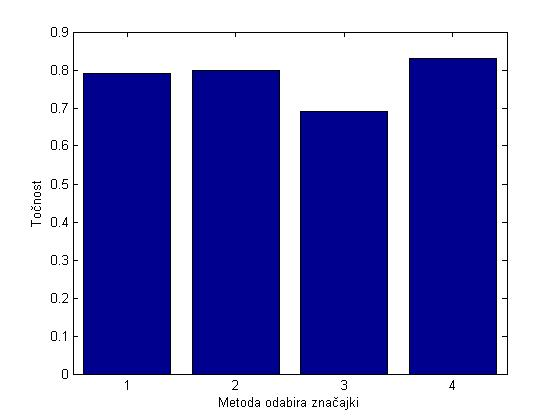
\includegraphics[width=\textwidth]{images/bayes.jpg}
\caption{Rezultati Naive Bayes metode}
\end{minipage}
\end{figure}

\begin{enumerate}
	\item Lista sentiment riječi (oko 6800 riječi)
	\item Riječi s najvećom frekvencijom (1000 riječi)
	\item Riječi s najvećom maksimalnom TF-IDF vrijednošću (1000 riječi)
	\item Najinformativnije značajke Naive Bayes klasifikatora (500 riječi)
\end{enumerate}



Ovisno o tome koje smo značajke uzimali, dobili smo sljedeće rezultate za linearni SVM:
\begin{itemize}
\item Za najfrekventnije značajke $78\%$
\item Za najinformativnije značajke $81\%$
\item Tf-idf - $70\%$
\item Lista sentiment riječi $83\%$
\end{itemize}
\section{Rezultati}
Možemo reći da nismo dobili očekivane rezultate. Očekivali smo da će metoda potpornih vektora bolje klasificirati od Naive-Bayes metode. Kod odabira značajki $tf-idf$ se pokazuje kao najgori. Pretpostavljamo da je to zbog toga što se one riječi koje su česte u svim dokumentima smatraju kao "zajedničke" i njihova "težina" (uloga) postaje manja. Tako na primjer ako se riječ $good$ pojavljuje u gotovo svim dokumentima $tf-idf$ će mu pridružiti težinu nula ($idf=\log \frac{\text{Ukupan broj dokumenata}}{\text{broj dokuemata u kojima se riječ pojavljuje}}$) pa će se taj pojam smatrati irelevantnim. Ipak SVM (linearan) daje ovdje bolje rezultate od naivnog Bayesa, kao i u slučaju uzimanja liste sentiment riječi.
\begin{thebibliography}{1}

\bibitem{thumbsup}
	B. Pang, L. Lee, S. Vaithyanathan,
 	Thumbs Up?: Sentiment Classification Using Machine Learning Techniques,
 	Proceedings of the ACL-02 Conference on Empirical Methods in Natural Language Processing - Volume 10,
 	Association for Computational Linguistics,
	Stroudsburg, PA, USA,
	2002.
	
\bibitem{stan}
	S. Jain, S. Nayak,
	Sentiment Analysis of Movie Reviews: A Study of Features and Classifiers\\
	\url{http://www.stanford.edu/~nayaks/reportsFolder/cs221_report.pdf}
	
\bibitem{uupp}
	M. Božić, I. Gavran,
	Analiza stava\\
	\url{http://stav.math.hr/static/data/uupp.pdf}
	
\bibitem{nltk}
	S. Bird, E. Klein, E. Loper,
	Natural Language Processing with Python,
	O'Reilly Media,
	2009.
	
\bibitem{tfidftutorial}
	S. Loria,
	Tutorial: Finding Important Words in Text Using TF-IDF\\
	\url{http://stevenloria.com/finding-important-words-in-a-document-using-tf-idf/}

\bibitem{dataset}
	B. Pang, L. Lee,
	Movie Review Data\\
	\url{https://www.cs.cornell.edu/people/pabo/movie-review-data/}
	
\bibitem{words}
	Opinion Lexicon (Sentiment Lexicon)\\
	\url{http://www.cs.uic.edu/~liub/FBS/sentiment-analysis.html#lexicon}
	
\bibitem{githubrepo}
	A. Kovačić, J. Marohnić, L. Arzon,
	Analiza stava u filmskim kritikama,
	GitHub repozitorij\\
	\url{https://github.com/janko-m/college-machine_learning}

\bibitem{scikit}
    Scikit-learn developeri,
    Support Vector Machines\\
    \url{http://scikit-learn.org/stable/modules/svm.html}

\end{thebibliography}

\end{document}
